\documentclass[]{article}


\usepackage[margin=1cm,includehead,landscape]{geometry}
\usepackage{fancyhdr}
\usepackage{multicol}
\usepackage{graphicx}
\pagestyle{fancy}
\usepackage{amsmath}
\usepackage{float}

\fancyhead[CO]{AdvElDes - Résumé 2021}
\fancyhead[LE,RO]{}
\fancyfoot[LE,RO]{}

\begin{document}
\begin{multicols}{3}
\section{Circuits}
\subsection{Amplificateurs opérationnels}
\subsubsection{GBW}
Produit constant sur la droite du GBW
$$A_0\cdot \omega_0 = \text{GBW}$$
Si on a une application avec $\omega_a$, alors le gain maximal est donné par
$$A_a=\frac{\text{GBW}}{\omega_a}$$
\subsubsection{Single supply, non inverting}
\begin{center}
\includegraphics[width=0.7\columnwidth,page=3]{../KiCad/resume-crop.pdf}
\end{center}
La valeur d'entrée $U_{in}$ est autour de 0. Le gain de tension est
$$G=\frac{R_2}{R_1}$$
Il n'y a pas de 1+, c'est normal. La valeur de sortie est autour de $U_{ref}$
\subsubsection{Single supply, inverting}
\begin{center}
\includegraphics[width=0.7\columnwidth,page=4]{../KiCad/resume-crop.pdf}
\end{center}
La tension d'entrée est autour de 0 et la tension de sortie est autour de $U_{ref}$
$$G=-\frac{R_1}{R_2}$$
\subsubsection{Single supply, differential}
\begin{center}
\includegraphics[width=0.7\columnwidth,page=5]{../KiCad/resume-crop.pdf}
\end{center}
$$G=2\frac{R_b}{R_a}$$
\section{Autres}
\subsection{Statistiques}
\begin{figure}[H]
\centering
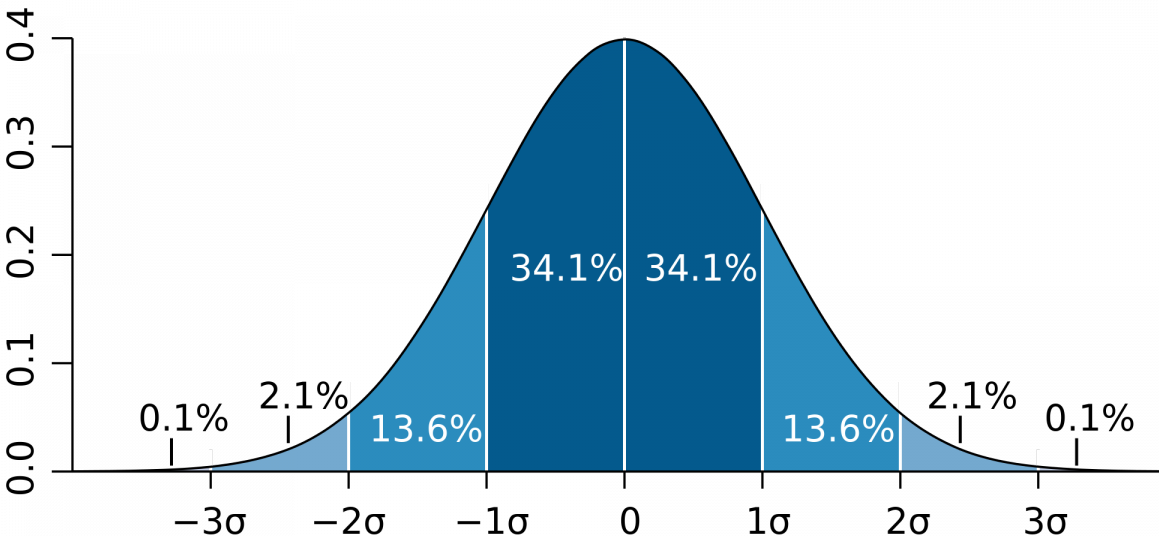
\includegraphics[width=0.6\columnwidth]{gauss.png}
\end{figure}

\end{multicols}





\end{document}